We proceed with the explanation of the implementation of \sys programming model, which is light and whose API adds very little on top of a plain C language.

\subsection{Application Programming Interface}
\label{sec:coala_api}

Coala's API adds only five syntactic constructs to a C-based language: (i) \texttt{COALA\_TASK}, to declare a new task, (ii) \texttt{COALA\_NEXT\_TASK}, to mark the next task to be run after the currently executing one completes, (iii) \texttt{COALA\_PV}, to declare a new protected variable, (iv) \texttt{RP} and \texttt{WP}, to mark protected variables' reads and writes, and (v) \texttt{COALA\_SM}, to declare \texttt{typedef}'d \texttt{struct} members, when used as protected variables, to ensure proper memory alignment required by \sys's page handler. Moreover, the programmer is required to explicitly call two API functions inside the main program body: (i) \texttt{COALA\_INIT}, to pass as an argument the global initialization task to run upon the first boot, and (ii) \texttt{COALA\_RUN}, which hands the control to \sys's task manager.

Table~\ref{table:coala_api} summarizes \sys's API methods and their arguments. \todo{Add example of a Coala program}{Carlo, Przemek} These methods trigger specific \sys kernel functions, whose explanation is given in the following sections.

\begin{table}
\centering
\begin{tabular}{| r | p{0.7\columnwidth} |}
	\hline
	{Method} & {Arguments} \\
	\hline\hline
	\texttt{COALA\_INIT}($t$) & $t \in \mathbf{T}$: task to be scheduled on the first boot \\
	\hline
	\texttt{COALA\_RUN}() & --- \\
	\hline
	\texttt{COALA\_TASK}($t$, $w_t$) & $t \in \mathbf{T}$: new task name, $w_t$: weight of task $t$ \\
	\hline
	\texttt{COALA\_NEXT\_TASK}($t$) & $t \in \mathbf{T}$ : task to be run next \\
	\hline
	\texttt{COALA\_PV}($p$, $v$ [, $s$]) & $p$: variable type, $v \in \mathbf{V}$: new protected variable name, $s$: array size \\
	\hline
	$u$ := \texttt{RP}($v$) & $v \in \mathbf{V}$: protected variable to be read, $u$: destination operand \\
	\hline	
	\texttt{WP}($v$) := $u$ &  $v \in \mathbf{V}$: protected variable to be written, $u$: source operand \\
	\hline
	\texttt{COALA\_SM}($p$, $m$ [, $s$]) & $p$: \texttt{struct} member's type, $m$: \texttt{struct} member's name, $s$: array size \\
	\hline
\end{tabular}
\caption{API summary; $\mathbf{T}$: set of all tasks, $\mathbf{V}$: set of all protected variables, $[, s]$: optional argument.}
\label{table:coala_api}
\end{table}

\subsection{Kernel Functions Implementation}

\textbf{New Tasks.} The API method \texttt{COALA\_TASK} statically allocates a non-volatile constant variable holding the task weight, and declares a void function with the name passed as an argument.

\textbf{New Protected Variables.} The API method \texttt{COALA\_PV} statically allocates (and aligns in memory) a non-volatile variable, whose address will be used by \texttt{RP} and \texttt{WP} API methods to locate the most recent location of the variable itself, which could be either the location of the variable in volatile memory or its location in non-volatile memory.

\textbf{Task Transitions.} By calling \texttt{COALA\_NEXT\_TASK}, the programmer tells \sys's task manager which task to execute next. The implementation of \sys is built on the assumption that the currently executing task is not interrupted, and only once it completes the next task is run.

\textbf{Protected Reads and Writes.} When \texttt{RP} and \texttt{WP} API methods are used, \sys searches the volatile memory for the page the protected variable belongs to. If such page is not found in RAM, then a page fault occurs, and the page is fetched from the non-volatile memory. The two functions return a handle to the variable's volatile memory location. Unlike \texttt{RP}, \texttt{WP} marks the page being written as dirty, so that it can be copied to its non-volatile location during the commit phase.

\textbf{Initialization and Origin Task.} The behavior of the API method \texttt{COALA\_INIT} is very similar to \texttt{COALA\_NEXT\_TASK}, with the addition that all the preliminary kernel initializations are performed inside this function. Moreover, the origin task is scheduled only upon the first boot.

\begin{wrapfigure}{t!}{0.5\textwidth}
	\centering
	%\includegraphics[width=0.5\columnwidth]{figures/graffle/state-machine.pdf}
	\caption{\sys state machine implementation \todo{Draw a figure}{Sinan, Carlo}}
	\label{fig:coala_state_machine}
\end{wrapfigure}

\noindent \textbf{Execution.} The application control is passed to \sys's execution manager by calling \texttt{COALA\_RUN} at the end of the main function. A high-level state machine of the execution manager is depicted in Figure~\ref{fig:coala_state_machine} \todo{Draw a figure reflecting the following description}{Sinan, Carlo}. Upon reboot, the coalescing target is initialized according to the coalescing strategy. Then, the second phase of the commit is resumed, in case the last power failure occurred during this operation. The shadow buffer list is cleared, and the metadata of the volatile buffer is initialized. The pointer to the last coalescing task is recalled from non-volatile memory. Before running, \sys checks whether there is any partial execution to resume, in which case the volatile state, including the program counter, is restored. Otherwise, coalescing starts: the current budget is replenished; tasks are run, the history is increased and the current budget is decreased; when the latter is zero, coalescing stops, the pointer to the next task is saved and the commit phase starts. Coalescing resumes after commit phase two ends and the target is updated based on the coalescing strategy. \todo{Go over keywords (coalescing target, current budget, commit phases etc.) and make them consistent with the rest of the paper}{Amjad, Carlo}

\subsection{Paging Implementation}

\sys's memory virtualization is implemented using three buffers: (i) working (volatile) buffer, (ii) store (non-volatile) buffer and (iii) shadow (non-volatile) buffer. The store buffer holds the latest safe copy of all the pages, and it is read-only up to, and including, the ultimate commit. Upon reboot, the working buffer is empty, and it gets filled with pages from non-volatile memory on demand. All reads and writes to protected variables happen in volatile memory. The shadow buffer serves as an intermediate non-volatile buffer where dirty, volatile pages are copied during the intermediate commit. Moreover, it contains pages evicted from SRAM when a \emph{full page fault} occurs.

\textbf{Page Allocation and Page Tags.} When a \sys application accesses a protected variable with either \texttt{RP} or \texttt{WP}, \sys has to search for the variable in RAM first, and then, if not found, in non-volatile memory. In reality, the page manager searches for pages, not single variables. A page search can be very fast if each page is identified by a unique tag, and if every variable belonging to a page bears the tag in its address. Thus, retrieving a page tag from a protected variable's address boils down to extracting the upper bits of the address itself. The remaining lower bits denote the variable's offset in its page. The complete process is depicted in Figure~\ref{figure:coala_page_tags} \todo{this figure doesn't really show page tags and offsets, but paging in general}.
We note that, in order to obtain unique page tags, some alignment requirements have to be met. First, the page size $S$ has to be the power of two. Moreover, pages in non-volatile memory have to be aligned by $S$. Note that, by aligning pages by $2^n$, the alignment is also valid for all sizes $2^x$, where $x \leq n$.

\begin{figure}
	\centering
	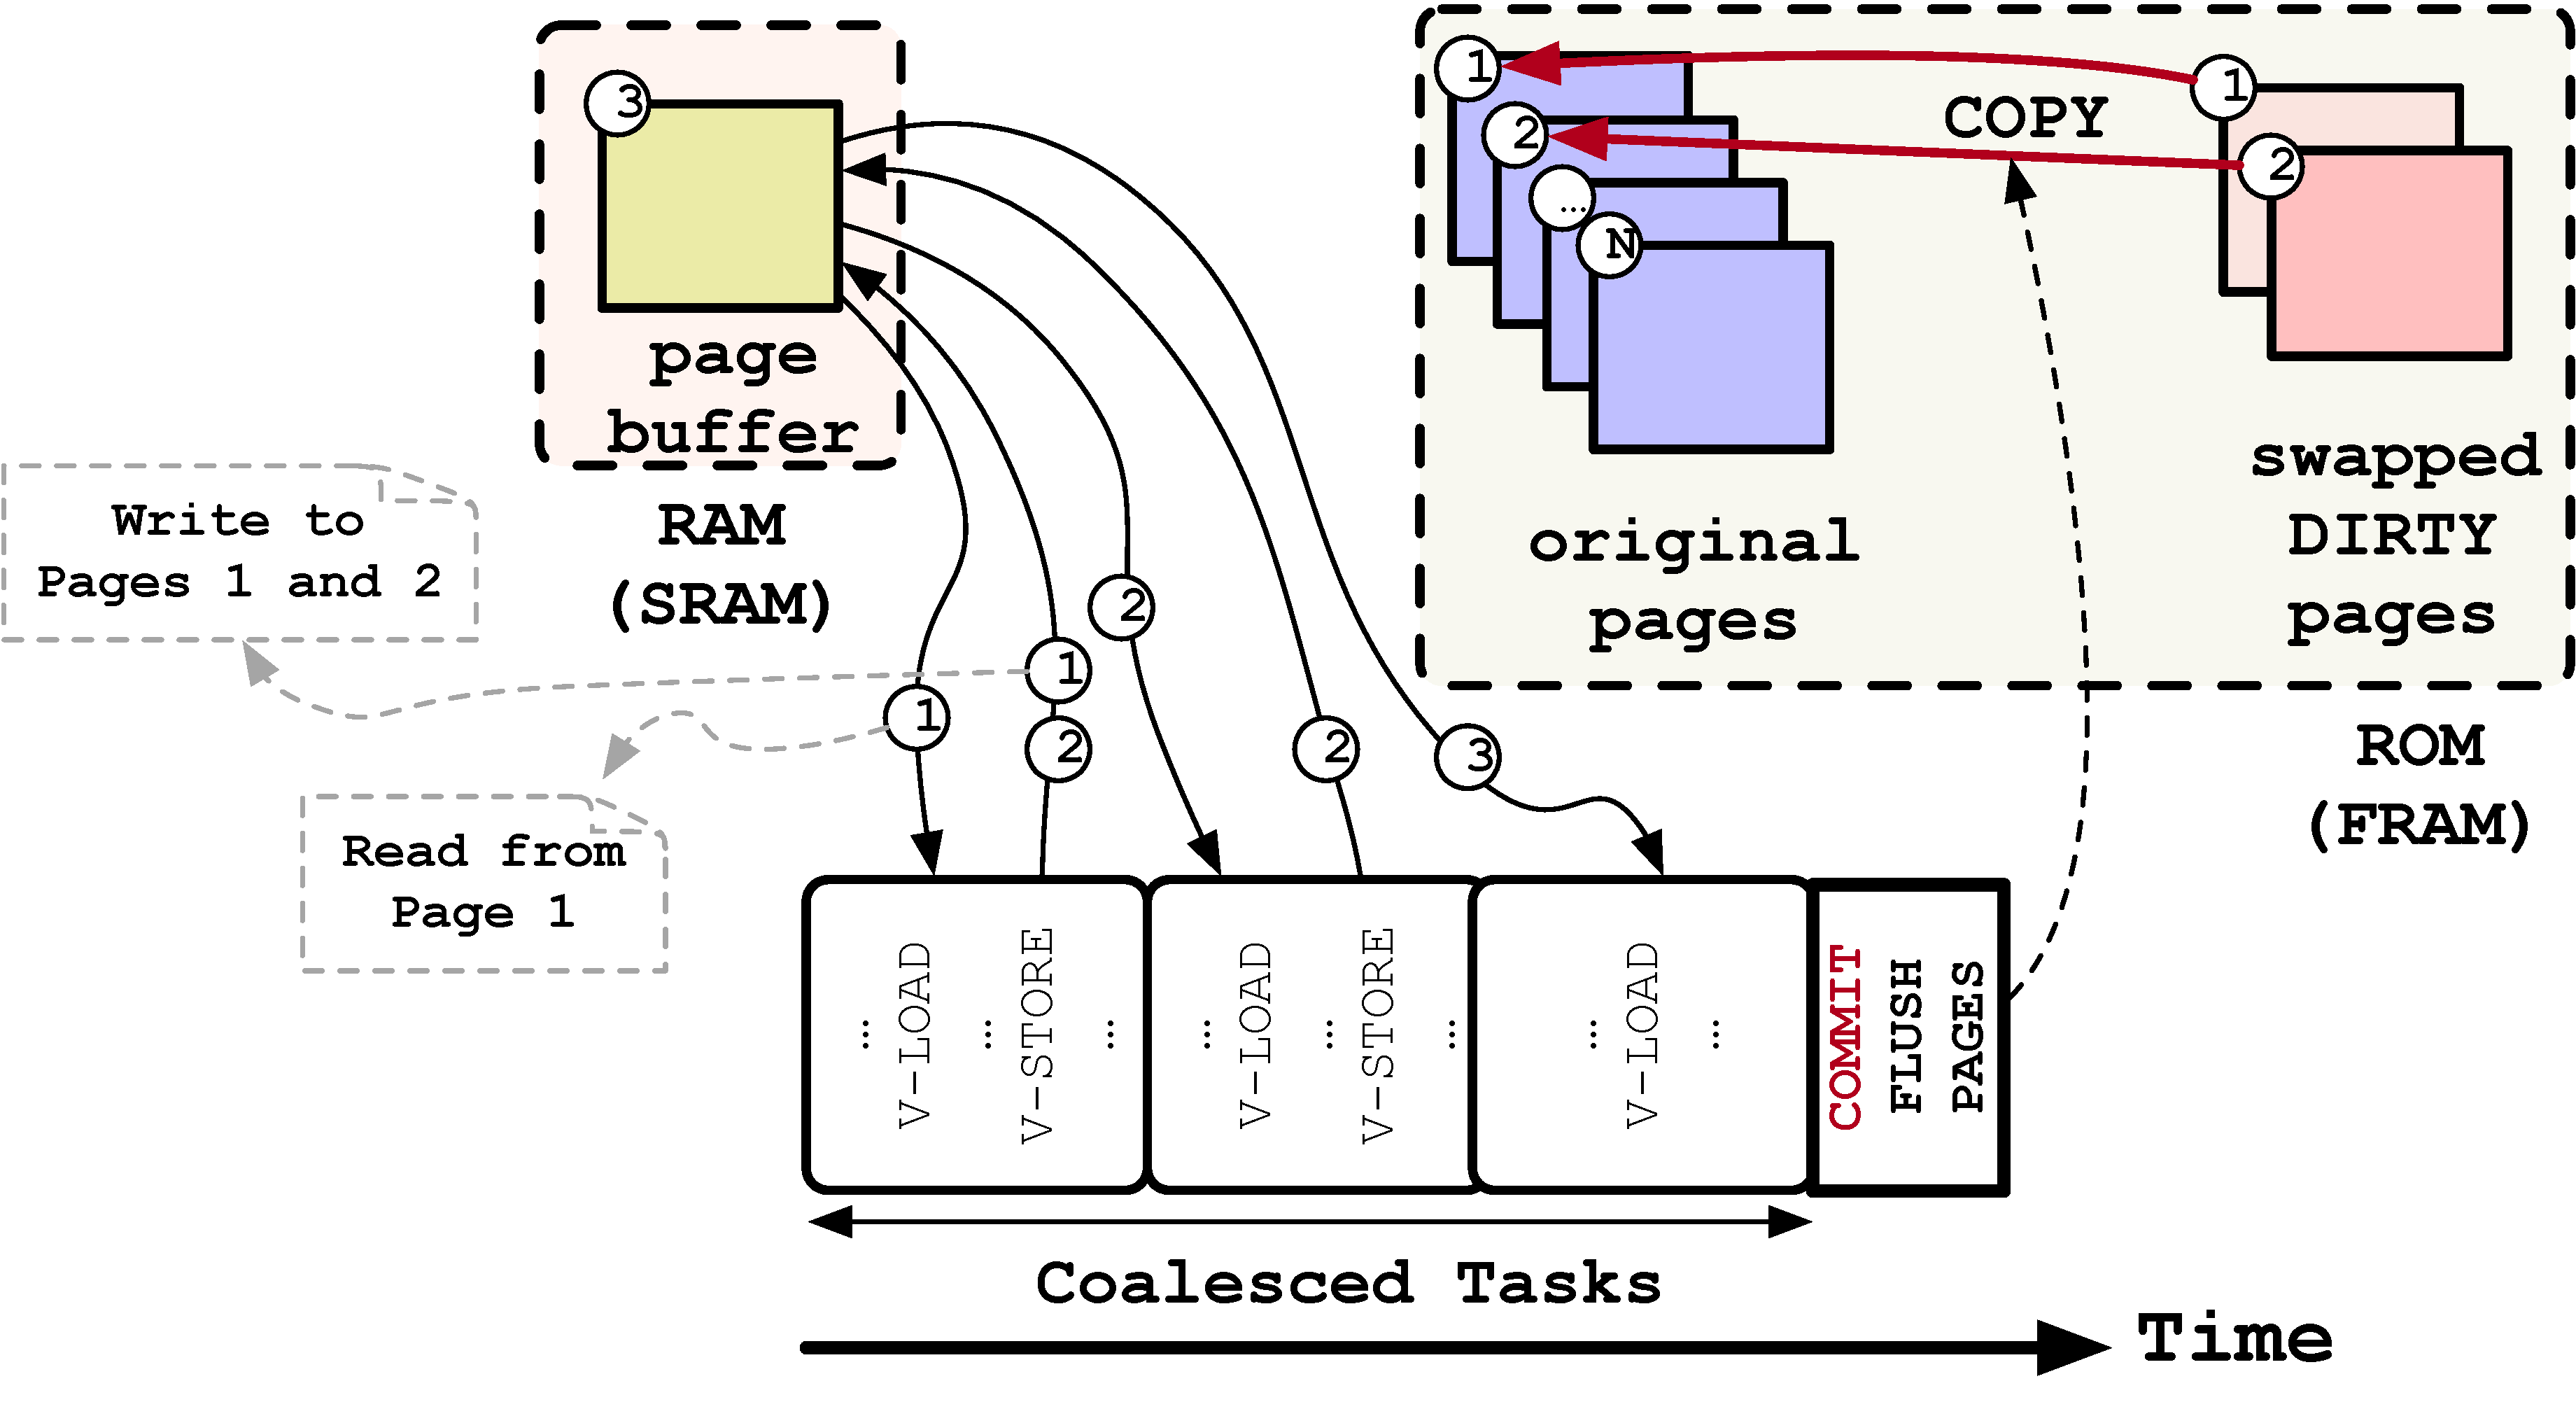
\includegraphics[width=\textwidth]{figures/graffle/paging.pdf}
	\caption{Illustration of \sys page tags mechanism.}
	\label{figure:coala_page_tags}
\end{figure}

\textbf{Page Fault and Page Swap.} When a page is not found in RAM, a \emph{page fault} it has to be fetched from FRAM. In case that page was in the working buffer and it had been evicted, its most recent non-volatile copy resides in the shadow buffer. For this reason, \sys searches this buffer first. If the requested page is not found in the shadow buffer, then it will be pulled from its store location. To make room for the requested page in SRAM, a volatile page might have to be evicted. If the victim page is dirty, we say that a \emph{full page fault} has occurred, and the victim page has to be copied to the shadow buffer. Page moves are accelerated by the MCU's direct memory access (DMA) module.

% It is important to mention that store and shadow buffers are virtual. By default, \sys allocates two memory banks for pages, $B0$ and $B1$, and all the pages have their store copy in $B0$. A dirty page that during the intermediate commit, or due to eviction, is copied to its shadow location in $B1$, will end up having its store location in $B1$ after the ultimate commit. Thus, during the ultimate commit

\subsection{Coalescing Loop and Commit Phase}

As described above, the main coalescing loop alternates between executing tasks and saving progresses. Static tasks are coalesced as long as the current budget is not null, after which the two commit phases are triggered, the coalescing target is updated and the current budget is replenished.

\textbf{Intermediate Commit and Ultimate Commit.} The reason why the commit process is split in two phases is two-fold: ensure consistency by using atomic operations, and preserving performance by enabling an incremental commit mechanism. When a coalesced task is successfully run to completion, all the dirty pages in SRAM have to be persistently saved to the non-volatile shadow buffer. This is what we call \emph{intermediate commit}: it has to be completed in one shot, and if power fails during this phase the application will have to resume from the beginning of the last coalesced task. When the intermediate commit is done, a flag can be atomically raised to signify that a valid, persistent copy of dirty pages is available in non-volatile memory. From this point on, the commit process can be resumed even if power fails.
To understand the last phase, referred to as \emph{ultimate commit}, it has to be mentioned that store and shadow buffers are virtual. By default, \sys allocates two memory banks for non-volatile pages, $M_0$ and $M_1$, and all the pages have their initial store copy in $M_0$. A dirty page that during the intermediate commit, or due to eviction, is copied to its shadow location in $M_x$, will end up having its store location in $M_x$ after the ultimate commit. In other words, during the ultimate commit dirty pages are not physically moved, instead their store and shadow locations are swapped. This trick makes \sys save some energy during this phase, avoiding redundant page moves. As for page swaps, the intermediate commit makes use of the on-board DMA.

\subsection{Partial execution}




\begin{wrapfigure}{t!}{0.5\textwidth}
	\centering
	%\includegraphics[width=0.5\columnwidth]{figures/graffle/commits-illustration.pdf}
	\caption{Intermediate commit and ultimate commit Illustration \todo{to be drawn}{sinan}}
	\label{fig:intermediate_ultimate-commit}
\end{wrapfigure}
